\section{Experimentación}

\subsection{Metodología}

\subsection{Test de tiempos}

Valores usados(Test de dimensions): \\
$m = 3$, $n = 3$, $r_i = 10$, $r_e = 100$, $ninst = 1$, $m$ y $n$ aumentan en 1. \\
Valores usados(Test de instancias): \\
$m = 15$, $n = 15$, $r_i = 10$, $r_e = 100$, $ninst = 1$, $ninst$ aumenta en 1. \\

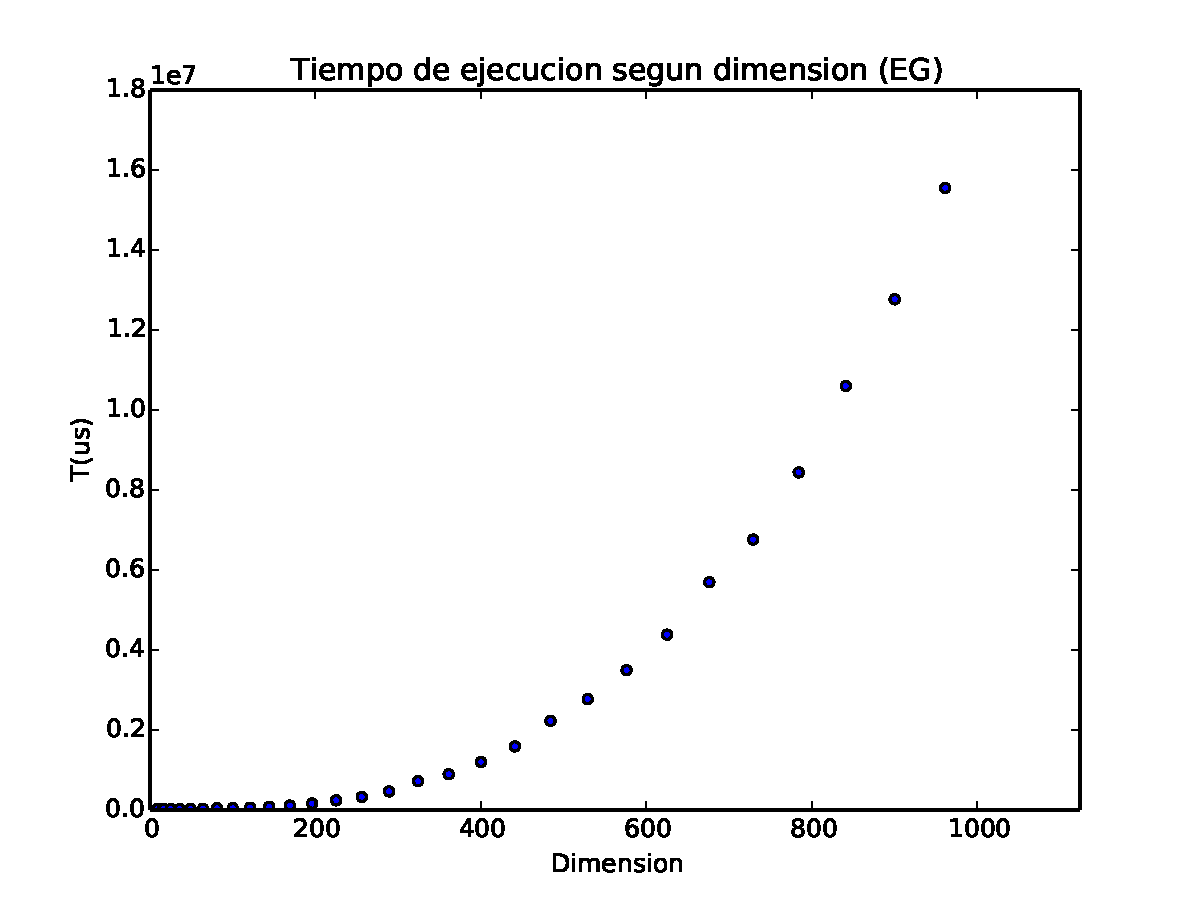
\includegraphics[scale=0.45]{graficos/dimVariable_EG.pdf}
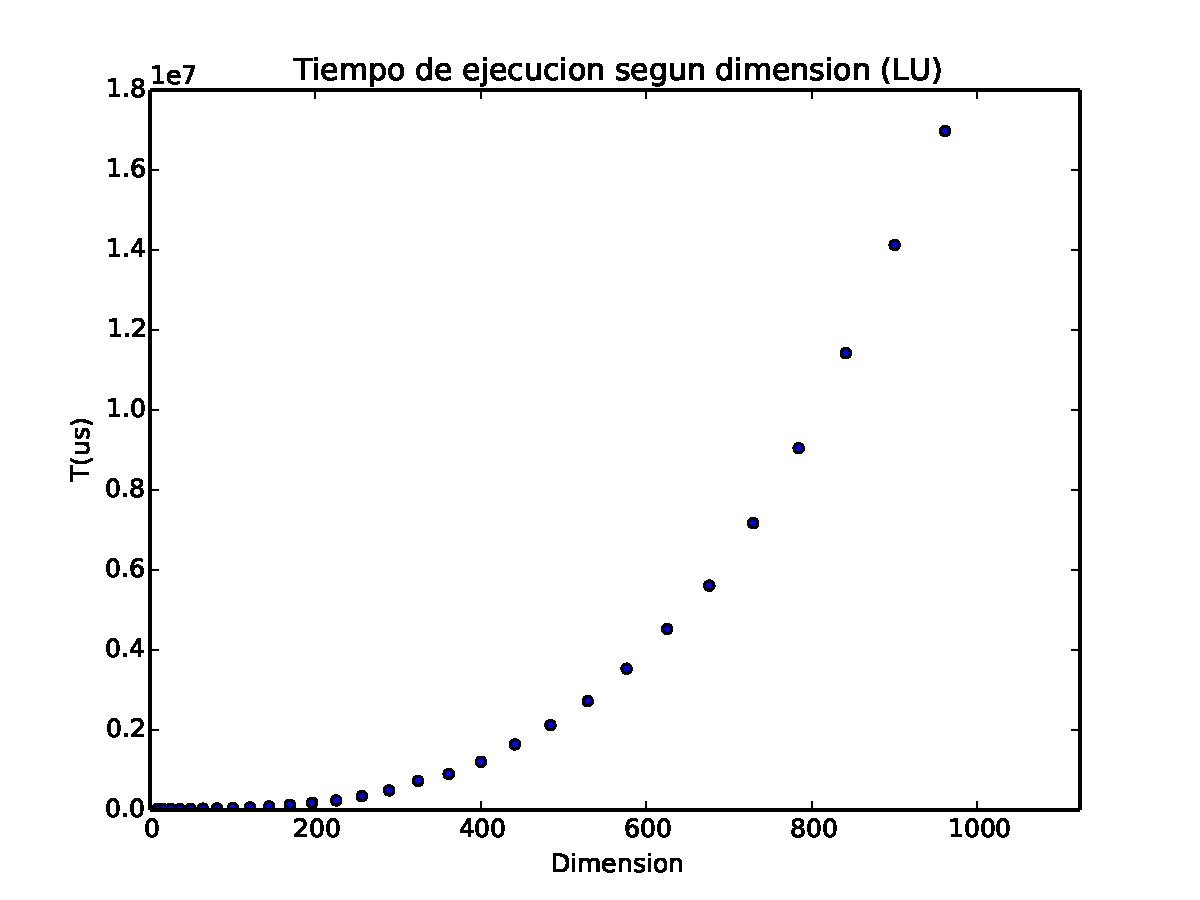
\includegraphics[scale=0.45]{graficos/dimVariable_LU.pdf}
\newline
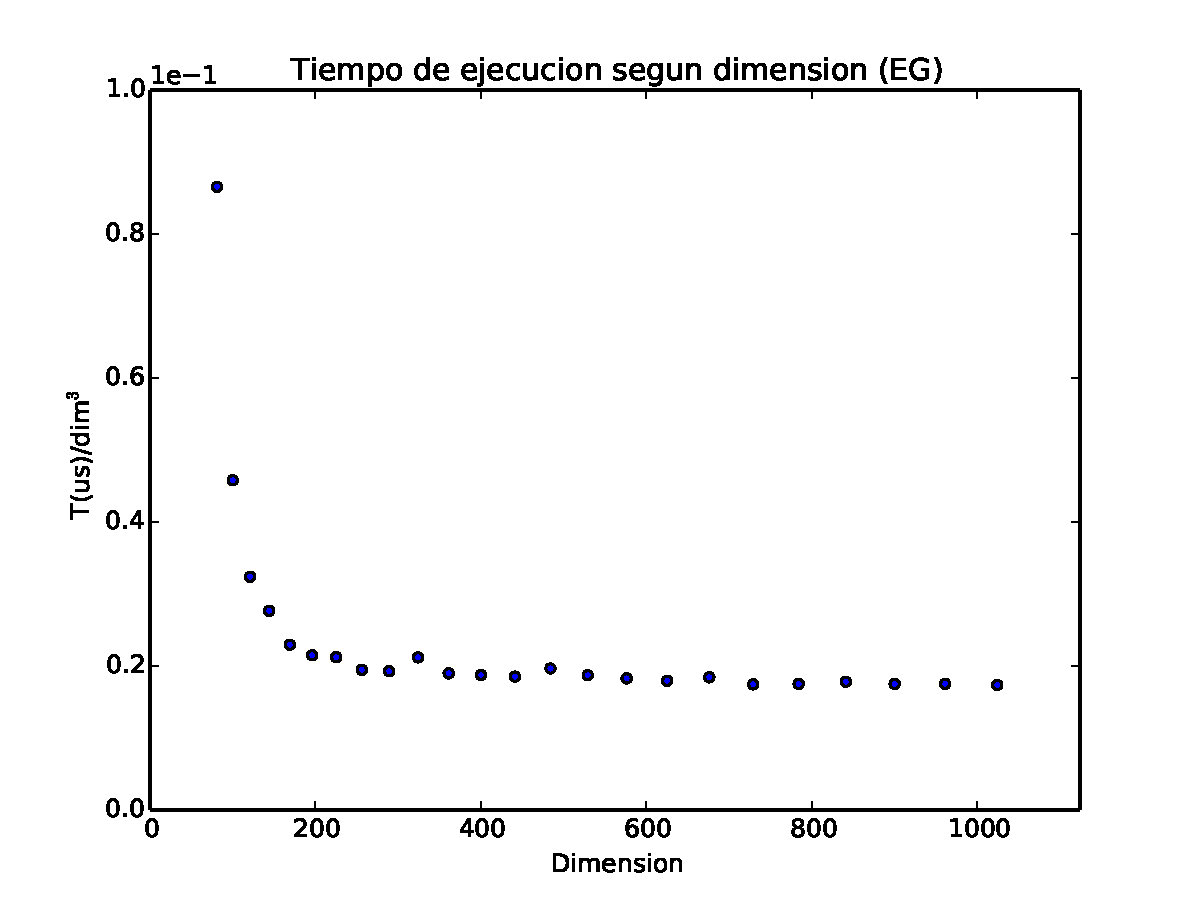
\includegraphics[scale=0.45]{graficos/dimVariableDiv_EG.pdf}
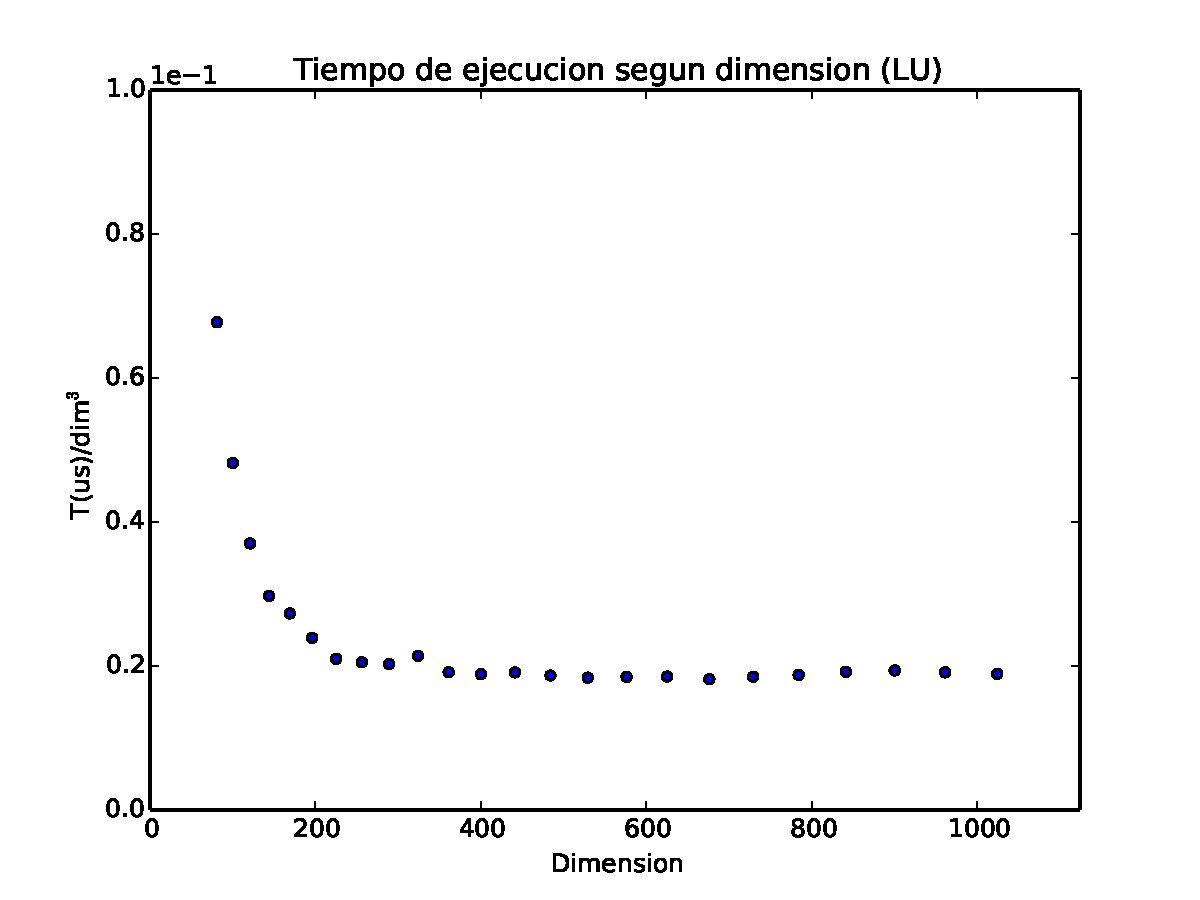
\includegraphics[scale=0.45]{graficos/dimVariableDiv_LU.pdf}
\newline
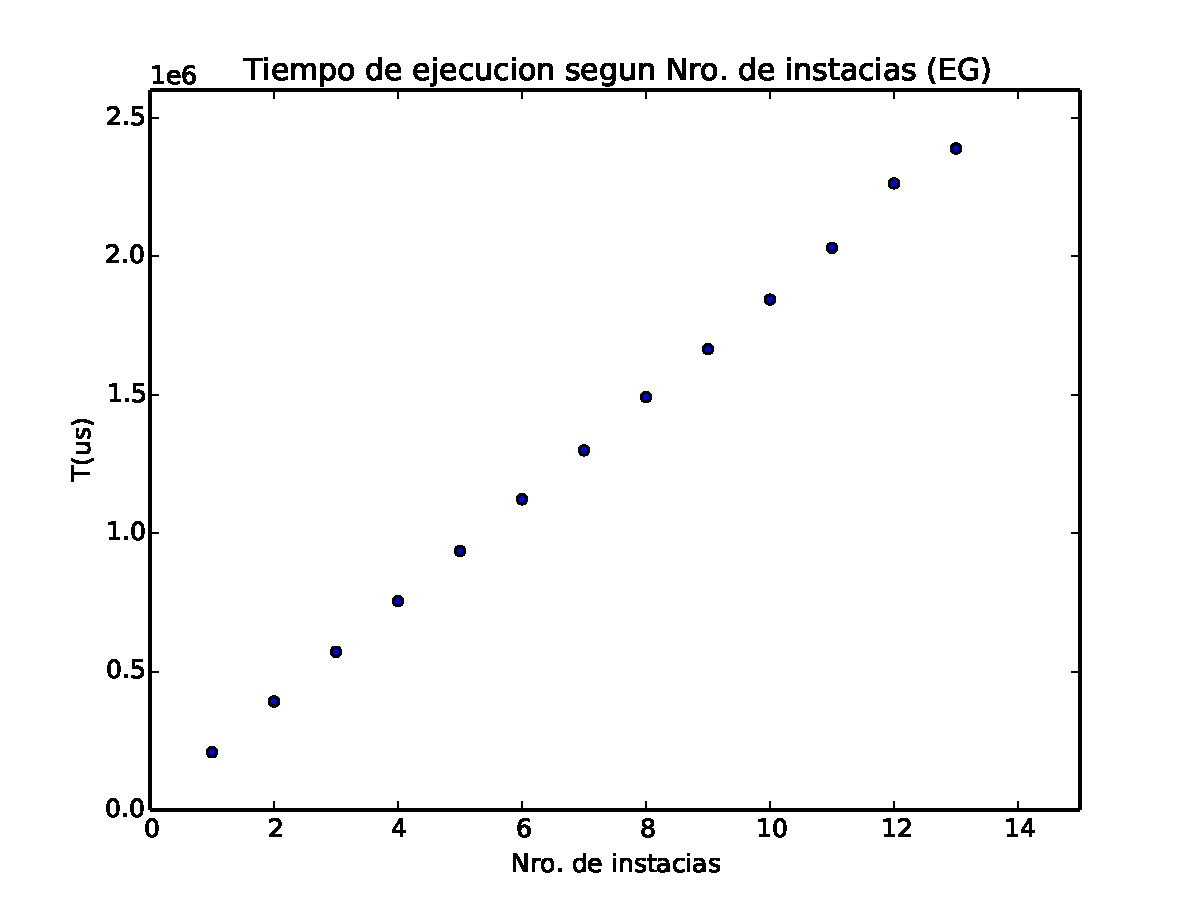
\includegraphics[scale=0.45]{graficos/instVariable_EG.pdf}
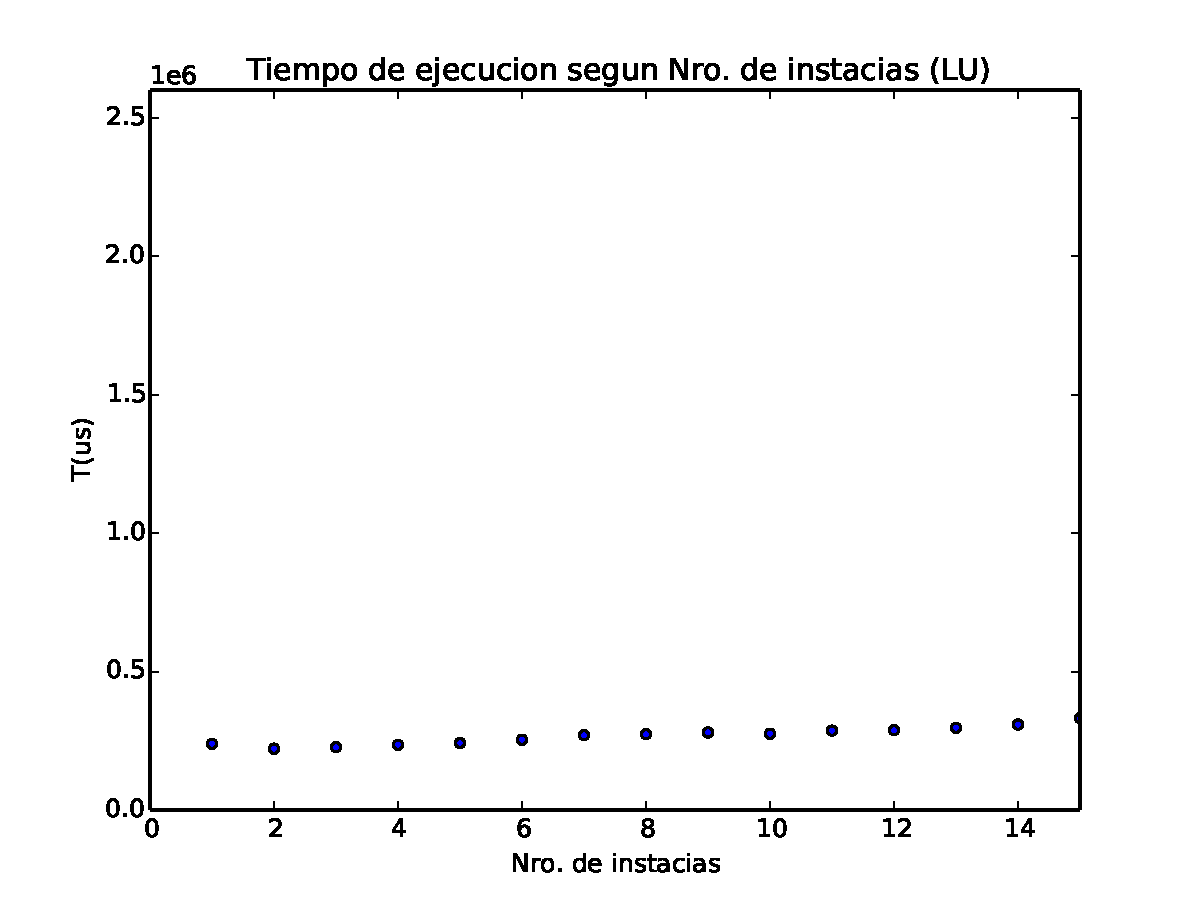
\includegraphics[scale=0.45]{graficos/instVariable_LU.pdf}

\begin{table}[]
\centering
\caption{Tiempo en obtener solucion (microsegundos)}
\label{tabla-eg-lu}
\begin{tabular}{lll}
\hline
Dim  & Tiempo(EG) & Tiempo(LU) \\ \hline
9    & 40000.0    & 24800.0    \\
16   & 26300.0    & 23300.0    \\
25   & 24700.0    & 23000.0    \\
36   & 25000.0    & 25200.0    \\
49   & 34500.0    & 31600.0    \\
64   & 30400.0    & 33600.0    \\
81   & 36300.0    & 40800.0    \\
100  & 42900.0    & 43900.0    \\
121  & 54500.0    & 59000.0    \\
144  & 75500.0    & 78300.0    \\
169  & 105400.0   & 110600.0   \\
196  & 147500.0   & 153100.0   \\
225  & 206800.0   & 215500.0   \\
256  & 292600.0   & 305200.0   \\
289  & 408000.0   & 427700.0   \\
324  & 574400.0   & 586600.0   \\
361  & 769000.0   & 808500.0   \\
400  & 1032500.0  & 1071700.0  \\
441  & 1368600.0  & 1423400.0  \\
484  & 1801900.0  & 1882200.0  \\
529  & 2338800.0  & 2454000.0  \\
576  & 3126600.0  & 3170100.0  \\
625  & 3850500.0  & 4073100.0  \\
676  & 4868300.0  & 5099500.0  \\
729  & 6115900.0  & 6420000.0  \\
784  & 7585900.0  & 7853900.0  \\
841  & 9363600.0  & 9725900.0  \\
900  & 11505200.0 & 12010300.0 \\
961  & 13940400.0 & 14459000.0 \\
1024 & 16863300.0 & 17570100.0 \\ \hline
\end{tabular}
\end{table}

\begin{table}[]
\centering
\caption{Tiempo en resolver todas las instacias (microsegundos)}
\label{tabla-instancias}
\begin{tabular}{lll}
\hline
Ninst & Tiempo(EG) & Tiempo(LU) \\ \hline
1     & 208600.0   & 238800.0   \\
2     & 391800.0   & 221400.0   \\
3     & 571500.0   & 227200.0   \\
4     & 754100.0   & 235200.0   \\
5     & 935400.0   & 242000.0   \\
6     & 1121900.0  & 253600.0   \\
7     & 1298700.0  & 270300.0   \\
8     & 1490800.0  & 274100.0   \\
9     & 1664000.0  & 280100.0   \\
10    & 1843100.0  & 275500.0   \\
11    & 2030100.0  & 286700.0   \\
12    & 2262700.0  & 288500.0   \\
13    & 2388500.0  & 296500.0   \\
14    & 2620200.0  & 308500.0   \\
15    & 2768700.0  & 331800.0   \\ \hline
\end{tabular}
\end{table}

\newpage
\subsection{Test de radios}

Valores usados: \\
$m = 8$, $n = 2$, $r_i = 10$, $r_e = 100$, $ninst = 1$, $epsilon$ para la convergencia $= 0.25$, $m$ aumenta en 4. \\

Izquierda: Metodo Lower, Derecha: Metdo Weighted \\

$r_i = 10$, $r_e = 100$ \\
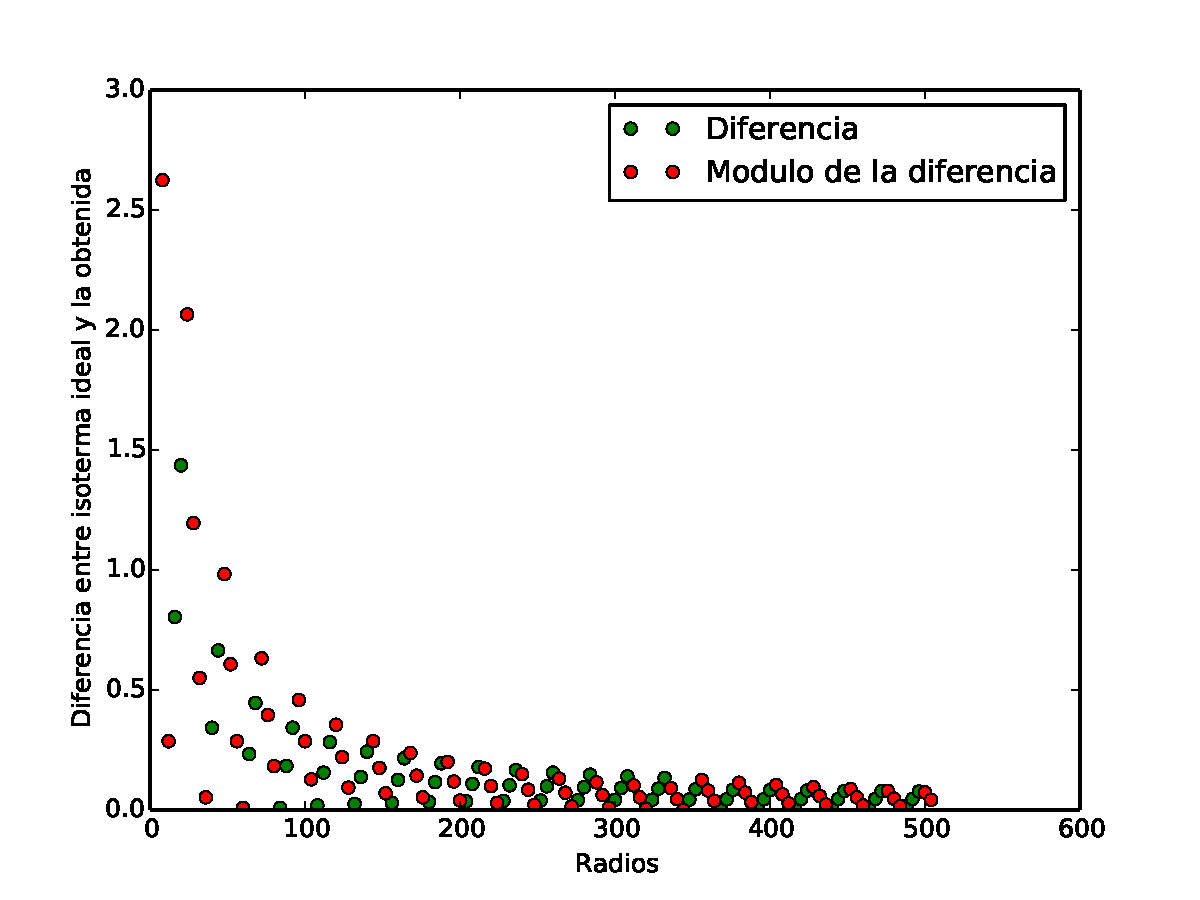
\includegraphics[scale=0.45]{graficos/mVariable_l_10_100.pdf}
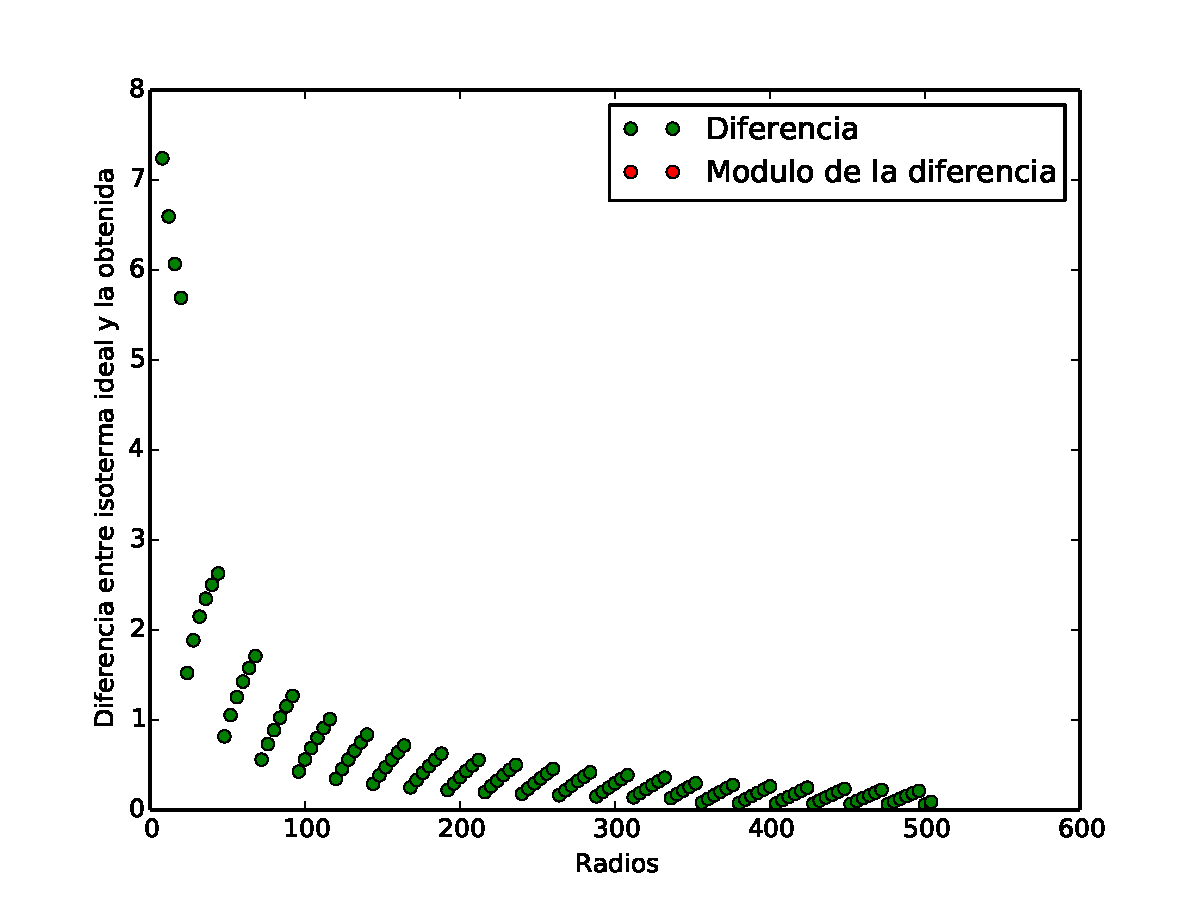
\includegraphics[scale=0.45]{graficos/mVariable_w_10_100.pdf}
\newline

$r_i = 25$, $r_e = 85$ \\
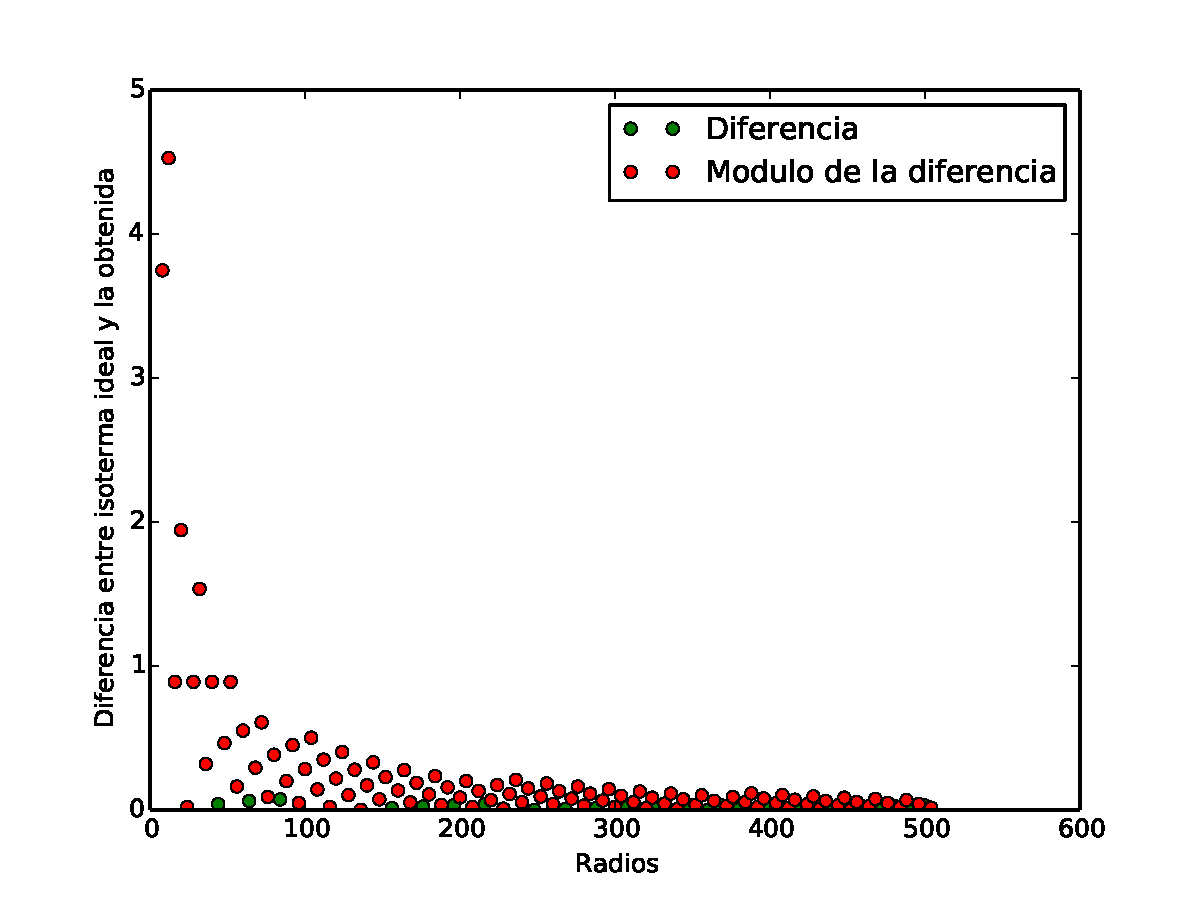
\includegraphics[scale=0.45]{graficos/mVariable_l_25_85.pdf}
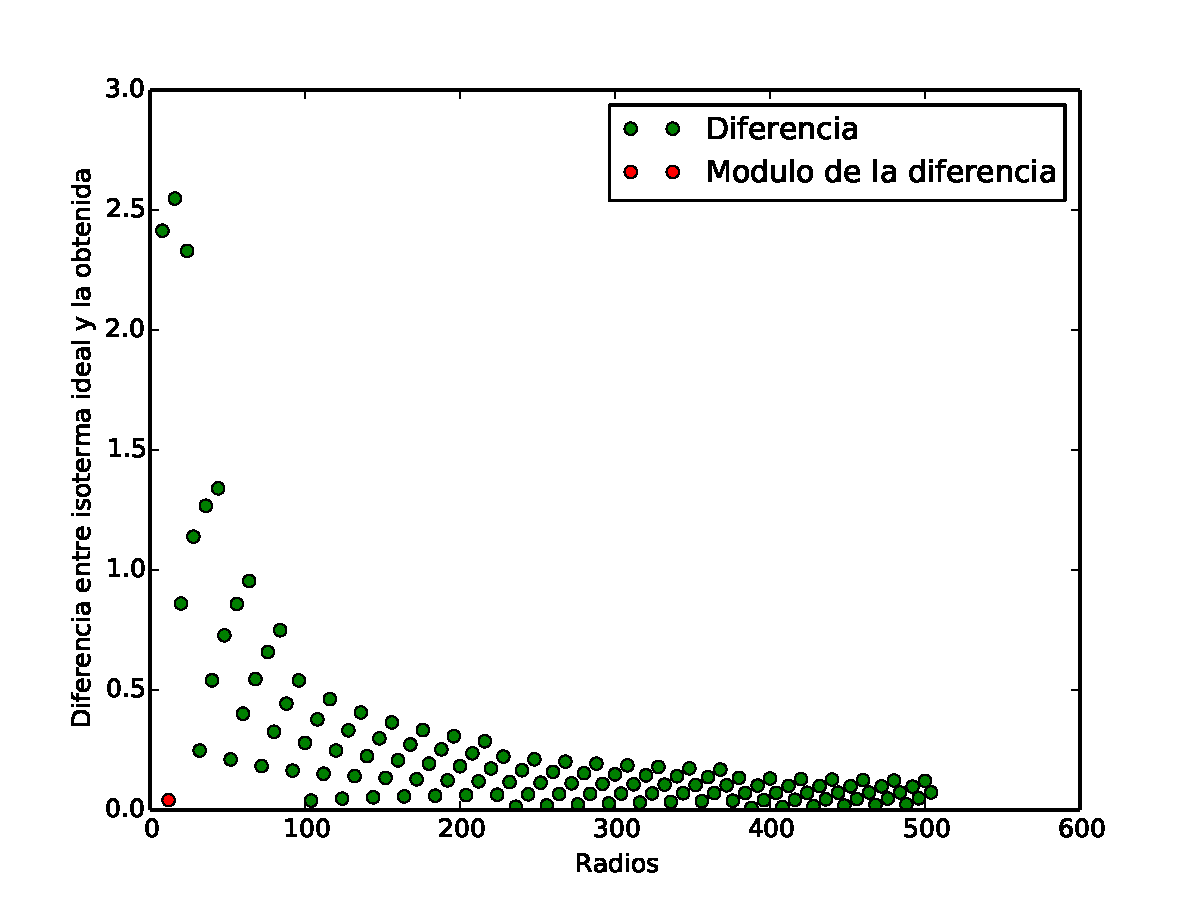
\includegraphics[scale=0.45]{graficos/mVariable_w_25_85.pdf}
\newline

$r_i = 40$, $r_e = 60$ \\
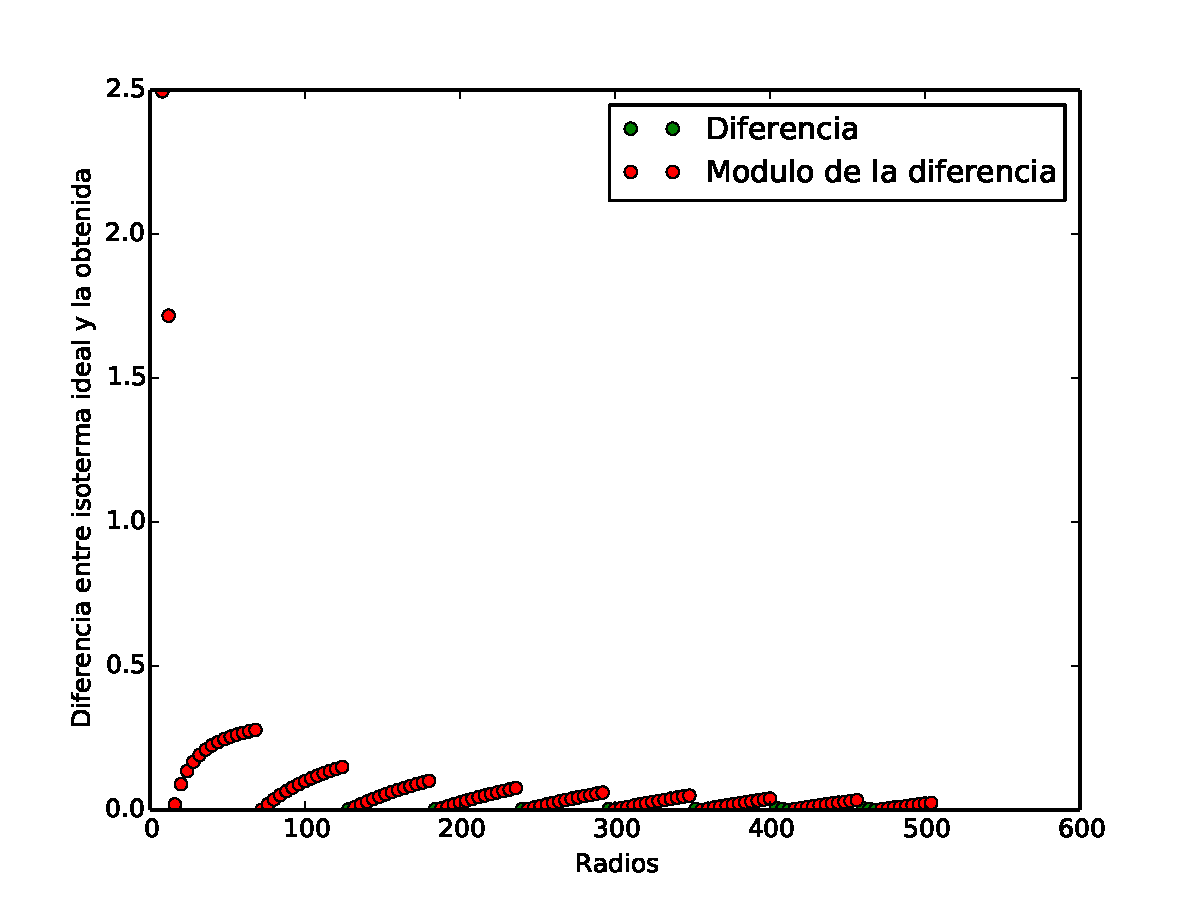
\includegraphics[scale=0.45]{graficos/mVariable_l_40_60.pdf}
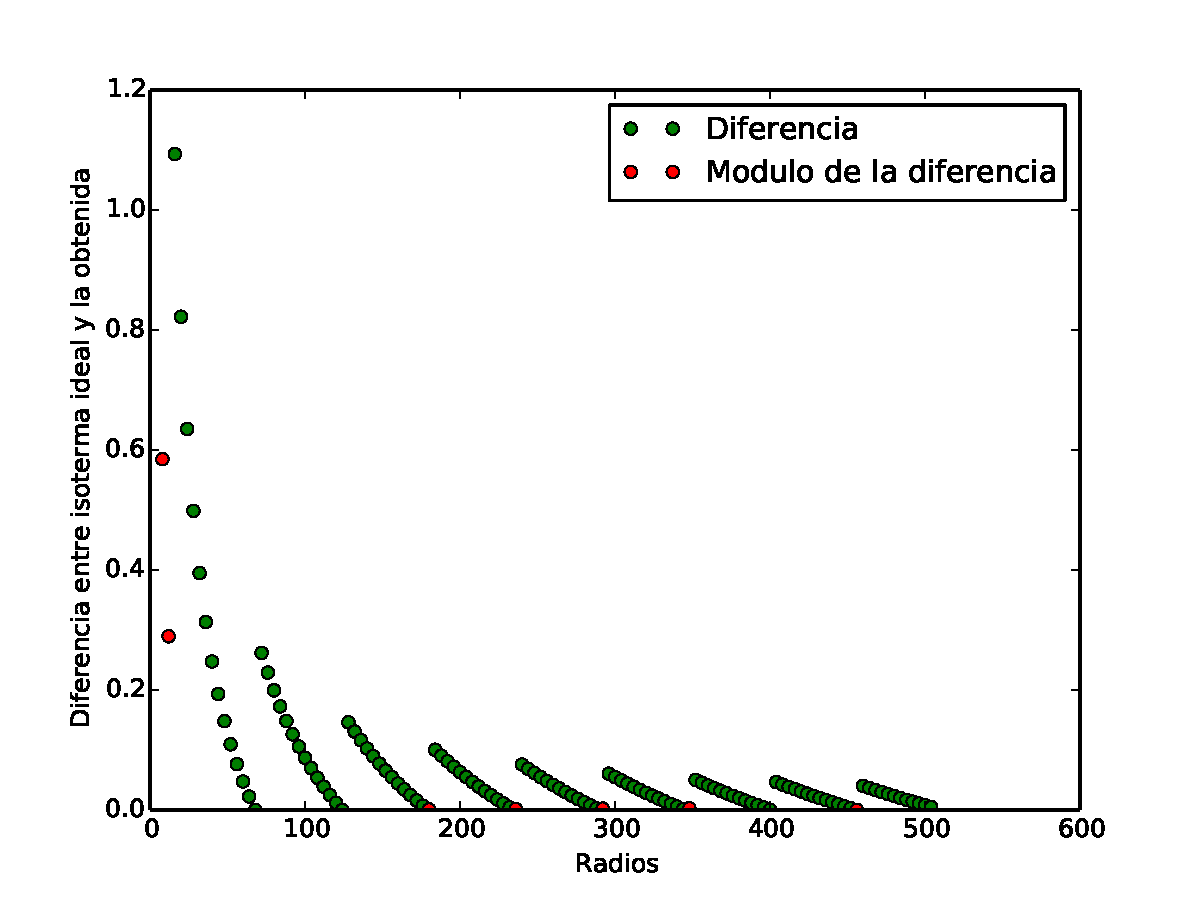
\includegraphics[scale=0.45]{graficos/mVariable_w_40_60.pdf}
\newline

\begin{table}[]
\centering
\caption{Valor de $m$ al partir del cual la solucion obtenida converge a la optima}
\label{tabla-metodos-isotermas}
\begin{tabular}{lll}
\hline
$\vert r_e - r_i \vert$ & Metodo Lower & Metodo Weighted \\ \hline
90                      & 144          & 400             \\
60                      & 164          & 216             \\
30                      & 68           & 72              \\ \hline
\end{tabular}
\end{table}

\subsection{Test de angulos}

$m = 20$, $n = 4$, $r_i = 10$, $r_e = 100$, $ninst = 1$, $m$ aumenta en 4. \\

\includegraphics[scale=0.5]{graficos/{nVariable_1.in_iso}.eps}
\includegraphics[scale=0.5]{graficos/{nVariable_2.in_iso}.eps}
\newline

\includegraphics[scale=0.5]{graficos/{nVariable_3.in_iso}.eps}
\includegraphics[scale=0.5]{graficos/{nVariable_4.in_iso}.eps}
\newline

\includegraphics[scale=0.5]{graficos/{nVariable_5.in_iso}.eps}
\newline

\subsection{Test de "no circularidad" de la Isoterma}

$m = 20$, $n = 20$, $r_i = 10$, $r_e = 100$, $ninst = 1$, $seed = 1520$ $temp\_ext$ aleatoria. \\

\includegraphics[scale=0.5]{graficos/{tempAleatoria_1.in_heat}.eps}
\includegraphics[scale=0.5]{graficos/{tempAleatoria_1.in_iso}.eps}
\newline

\includegraphics[scale=0.5]{graficos/{tempAleatoria_2.in_heat}.eps}
\includegraphics[scale=0.5]{graficos/{tempAleatoria_2.in_iso}.eps}
\newline

\includegraphics[scale=0.5]{graficos/{tempAleatoria_3.in_heat}.eps}
\includegraphics[scale=0.5]{graficos/{tempAleatoria_3.in_iso}.eps}
\newline


